
%% bare_jrnl.tex
%% V1.3
%% 2007/01/11
%% by Michael Shell
%% see http://www.michaelshell.org/
%% for current contact information.
%%
%% This is a skeleton file demonstrating the use of IEEEtran.cls
%% (requires IEEEtran.cls version 1.7 or later) with an IEEE journal paper.
%%
%% Support sites:
%% http://www.michaelshell.org/tex/ieeetran/
%% http://www.ctan.org/tex-archive/macros/latex/contrib/IEEEtran/
%% and
%% http://www.ieee.org/



% *** Authors should verify (and, if needed, correct) their LaTeX system  ***
% *** with the testflow diagnostic prior to trusting their LaTeX platform ***
% *** with production work. IEEE's font choices can trigger bugs that do  ***
% *** not appear when using other class files.                            ***
% The testflow support page is at:
% http://www.michaelshell.org/tex/testflow/


%%*************************************************************************
%% Legal Notice:
%% This code is offered as-is without any warranty either expressed or
%% implied; without even the implied warranty of MERCHANTABILITY or
%% FITNESS FOR A PARTICULAR PURPOSE! 
%% User assumes all risk.
%% In no event shall IEEE or any contributor to this code be liable for
%% any damages or losses, including, but not limited to, incidental,
%% consequential, or any other damages, resulting from the use or misuse
%% of any information contained here.
%%
%% All comments are the opinions of their respective authors and are not
%% necessarily endorsed by the IEEE.
%%
%% This work is distributed under the LaTeX Project Public License (LPPL)
%% ( http://www.latex-project.org/ ) version 1.3, and may be freely used,
%% distributed and modified. A copy of the LPPL, version 1.3, is included
%% in the base LaTeX documentation of all distributions of LaTeX released
%% 2003/12/01 or later.
%% Retain all contribution notices and credits.
%% ** Modified files should be clearly indicated as such, including  **
%% ** renaming them and changing author support contact information. **
%%
%% File list of work: IEEEtran.cls, IEEEtran_HOWTO.pdf, bare_adv.tex,
%%                    bare_conf.tex, bare_jrnl.tex, bare_jrnl_compsoc.tex
%%*************************************************************************

% Note that the a4paper option is mainly intended so that authors in
% countries using A4 can easily print to A4 and see how their papers will
% look in print - the typesetting of the document will not typically be
% affected with changes in paper size (but the bottom and side margins will).
% Use the testflow package mentioned above to verify correct handling of
% both paper sizes by the user's LaTeX system.
%
% Also note that the "draftcls" or "draftclsnofoot", not "draft", option
% should be used if it is desired that the figures are to be displayed in
% draft mode.
%
\documentclass[journal]{IEEEtran}
%
% If IEEEtran.cls has not been installed into the LaTeX system files,
% manually specify the path to it like:
% \documentclass[journal]{../sty/IEEEtran}





% Some very useful LaTeX packages include:
% (uncomment the ones you want to load)


% *** MISC UTILITY PACKAGES ***
%
%\usepackage{ifpdf}
% Heiko Oberdiek's ifpdf.sty is very useful if you need conditional
% compilation based on whether the output is pdf or dvi.
% usage:
% \ifpdf
%   % pdf code
% \else
%   % dvi code
% \fi
% The latest version of ifpdf.sty can be obtained from:
% http://www.ctan.org/tex-archive/macros/latex/contrib/oberdiek/
% Also, note that IEEEtran.cls V1.7 and later provides a builtin
% \ifCLASSINFOpdf conditional that works the same way.
% When switching from latex to pdflatex and vice-versa, the compiler may
% have to be run twice to clear warning/error messages.


% *** GRAPHICS RELATED PACKAGES ***
%
 \usepackage[pdftex]{graphicx}
 \graphicspath{{images/}}
  
% graphicx was written by David Carlisle and Sebastian Rahtz. It is
% required if you want graphics, photos, etc. graphicx.sty is already
% installed on most LaTeX systems. The latest version and documentation can
% be obtained at: 
% http://www.ctan.org/tex-archive/macros/latex/required/graphics/
% Another good source of documentation is "Using Imported Graphics in
% LaTeX2e" by Keith Reckdahl which can be found as epslatex.ps or
% epslatex.pdf at: http://www.ctan.org/tex-archive/info/
%
% latex, and pdflatex in dvi mode, support graphics in encapsulated
% postscript (.eps) format. pdflatex in pdf mode supports graphics
% in .pdf, .jpeg, .png and .mps (metapost) formats. Users should ensure
% that all non-photo figures use a vector format (.eps, .pdf, .mps) and
% not a bitmapped formats (.jpeg, .png). IEEE frowns on bitmapped formats
% which can result in "jaggedy"/blurry rendering of lines and letters as
% well as large increases in file sizes.
%
% You can find documentation about the pdfTeX application at:
% http://www.tug.org/applications/pdftex





% *** MATH PACKAGES ***
%
%\usepackage[cmex10]{amsmath}
% A popular package from the American Mathematical Society that provides
% many useful and powerful commands for dealing with mathematics. If using
% it, be sure to load this package with the cmex10 option to ensure that
% only type 1 fonts will utilized at all point sizes. Without this option,
% it is possible that some math symbols, particularly those within
% footnotes, will be rendered in bitmap form which will result in a
% document that can not be IEEE Xplore compliant!
%
% Also, note that the amsmath package sets \interdisplaylinepenalty to 10000
% thus preventing page breaks from occurring within multiline equations. Use:
%\interdisplaylinepenalty=2500
% after loading amsmath to restore such page breaks as IEEEtran.cls normally
% does. amsmath.sty is already installed on most LaTeX systems. The latest
% version and documentation can be obtained at:
% http://www.ctan.org/tex-archive/macros/latex/required/amslatex/math/





% *** SPECIALIZED LIST PACKAGES ***
%
%\usepackage{algorithmic}
% algorithmic.sty was written by Peter Williams and Rogerio Brito.
% This package provides an algorithmic environment fo describing algorithms.
% You can use the algorithmic environment in-text or within a figure
% environment to provide for a floating algorithm. Do NOT use the algorithm
% floating environment provided by algorithm.sty (by the same authors) or
% algorithm2e.sty (by Christophe Fiorio) as IEEE does not use dedicated
% algorithm float types and packages that provide these will not provide
% correct IEEE style captions. The latest version and documentation of
% algorithmic.sty can be obtained at:
% http://www.ctan.org/tex-archive/macros/latex/contrib/algorithms/
% There is also a support site at:
% http://algorithms.berlios.de/index.html
% Also of interest may be the (relatively newer and more customizable)
% algorithmicx.sty package by Szasz Janos:
% http://www.ctan.org/tex-archive/macros/latex/contrib/algorithmicx/




% *** ALIGNMENT PACKAGES ***
%
%\usepackage{array}
% Frank Mittelbach's and David Carlisle's array.sty patches and improves
% the standard LaTeX2e array and tabular environments to provide better
% appearance and additional user controls. As the default LaTeX2e table
% generation code is lacking to the point of almost being broken with
% respect to the quality of the end results, all users are strongly
% advised to use an enhanced (at the very least that provided by array.sty)
% set of table tools. array.sty is already installed on most systems. The
% latest version and documentation can be obtained at:
% http://www.ctan.org/tex-archive/macros/latex/required/tools/


%\usepackage{mdwmath}
%\usepackage{mdwtab}
% Also highly recommended is Mark Wooding's extremely powerful MDW tools,
% especially mdwmath.sty and mdwtab.sty which are used to format equations
% and tables, respectively. The MDWtools set is already installed on most
% LaTeX systems. The lastest version and documentation is available at:
% http://www.ctan.org/tex-archive/macros/latex/contrib/mdwtools/


% IEEEtran contains the IEEEeqnarray family of commands that can be used to
% generate multiline equations as well as matrices, tables, etc., of high
% quality.


%\usepackage{eqparbox}
% Also of notable interest is Scott Pakin's eqparbox package for creating
% (automatically sized) equal width boxes - aka "natural width parboxes".
% Available at:
% http://www.ctan.org/tex-archive/macros/latex/contrib/eqparbox/





% *** SUBFIGURE PACKAGES ***
%\usepackage[tight,footnotesize]{subfigure}
% subfigure.sty was written by Steven Douglas Cochran. This package makes it
% easy to put subfigures in your figures. e.g., "Figure 1a and 1b". For IEEE
% work, it is a good idea to load it with the tight package option to reduce
% the amount of white space around the subfigures. subfigure.sty is already
% installed on most LaTeX systems. The latest version and documentation can
% be obtained at:
% http://www.ctan.org/tex-archive/obsolete/macros/latex/contrib/subfigure/
% subfigure.sty has been superceeded by subfig.sty.



%\usepackage[caption=false]{caption}
%\usepackage[font=footnotesize]{subfig}
% subfig.sty, also written by Steven Douglas Cochran, is the modern
% replacement for subfigure.sty. However, subfig.sty requires and
% automatically loads Axel Sommerfeldt's caption.sty which will override
% IEEEtran.cls handling of captions and this will result in nonIEEE style
% figure/table captions. To prevent this problem, be sure and preload
% caption.sty with its "caption=false" package option. This is will preserve
% IEEEtran.cls handing of captions. Version 1.3 (2005/06/28) and later 
% (recommended due to many improvements over 1.2) of subfig.sty supports
% the caption=false option directly:
%\usepackage[caption=false,font=footnotesize]{subfig}
%
% The latest version and documentation can be obtained at:
% http://www.ctan.org/tex-archive/macros/latex/contrib/subfig/
% The latest version and documentation of caption.sty can be obtained at:
% http://www.ctan.org/tex-archive/macros/latex/contrib/caption/




% *** FLOAT PACKAGES ***
%
%\usepackage{fixltx2e}
% fixltx2e, the successor to the earlier fix2col.sty, was written by
% Frank Mittelbach and David Carlisle. This package corrects a few problems
% in the LaTeX2e kernel, the most notable of which is that in current
% LaTeX2e releases, the ordering of single and double column floats is not
% guaranteed to be preserved. Thus, an unpatched LaTeX2e can allow a
% single column figure to be placed prior to an earlier double column
% figure. The latest version and documentation can be found at:
% http://www.ctan.org/tex-archive/macros/latex/base/



%\usepackage{stfloats}
% stfloats.sty was written by Sigitas Tolusis. This package gives LaTeX2e
% the ability to do double column floats at the bottom of the page as well
% as the top. (e.g., "\begin{figure*}[!b]" is not normally possible in
% LaTeX2e). It also provides a command:
%\fnbelowfloat
% to enable the placement of footnotes below bottom floats (the standard
% LaTeX2e kernel puts them above bottom floats). This is an invasive package
% which rewrites many portions of the LaTeX2e float routines. It may not work
% with other packages that modify the LaTeX2e float routines. The latest
% version and documentation can be obtained at:
% http://www.ctan.org/tex-archive/macros/latex/contrib/sttools/
% Documentation is contained in the stfloats.sty comments as well as in the
% presfull.pdf file. Do not use the stfloats baselinefloat ability as IEEE
% does not allow \baselineskip to stretch. Authors submitting work to the
% IEEE should note that IEEE rarely uses double column equations and
% that authors should try to avoid such use. Do not be tempted to use the
% cuted.sty or midfloat.sty packages (also by Sigitas Tolusis) as IEEE does
% not format its papers in such ways.


%\ifCLASSOPTIONcaptionsoff
%  \usepackage[nomarkers]{endfloat}
% \let\MYoriglatexcaption\caption
% \renewcommand{\caption}[2][\relax]{\MYoriglatexcaption[#2]{#2}}
%\fi
% endfloat.sty was written by James Darrell McCauley and Jeff Goldberg.
% This package may be useful when used in conjunction with IEEEtran.cls'
% captionsoff option. Some IEEE journals/societies require that submissions
% have lists of figures/tables at the end of the paper and that
% figures/tables without any captions are placed on a page by themselves at
% the end of the document. If needed, the draftcls IEEEtran class option or
% \CLASSINPUTbaselinestretch interface can be used to increase the line
% spacing as well. Be sure and use the nomarkers option of endfloat to
% prevent endfloat from "marking" where the figures would have been placed
% in the text. The two hack lines of code above are a slight modification of
% that suggested by in the endfloat docs (section 8.3.1) to ensure that
% the full captions always appear in the list of figures/tables - even if
% the user used the short optional argument of \caption[]{}.
% IEEE papers do not typically make use of \caption[]'s optional argument,
% so this should not be an issue. A similar trick can be used to disable
% captions of packages such as subfig.sty that lack options to turn off
% the subcaptions:
% For subfig.sty:
% \let\MYorigsubfloat\subfloat
% \renewcommand{\subfloat}[2][\relax]{\MYorigsubfloat[]{#2}}
% For subfigure.sty:
% \let\MYorigsubfigure\subfigure
% \renewcommand{\subfigure}[2][\relax]{\MYorigsubfigure[]{#2}}
% However, the above trick will not work if both optional arguments of
% the \subfloat/subfig command are used. Furthermore, there needs to be a
% description of each subfigure *somewhere* and endfloat does not add
% subfigure captions to its list of figures. Thus, the best approach is to
% avoid the use of subfigure captions (many IEEE journals avoid them anyway)
% and instead reference/explain all the subfigures within the main caption.
% The latest version of endfloat.sty and its documentation can obtained at:
% http://www.ctan.org/tex-archive/macros/latex/contrib/endfloat/
%
% The IEEEtran \ifCLASSOPTIONcaptionsoff conditional can also be used
% later in the document, say, to conditionally put the References on a 
% page by themselves.


\usepackage{biblatex}
\usepackage[pdfborder={0 0 0}]{hyperref}
\bibliography{literature}

% correct bad hyphenation here
\hyphenation{op-tical net-works semi-conduc-tor}


\begin{document}
%
% paper title
% can use linebreaks \\ within to get better formatting as desired
\title{Simulation with OMNeT++ in real time}
%
%
% author names and IEEE memberships
% note positions of commas and nonbreaking spaces ( ~ ) LaTeX will not break
% a structure at a ~ so this keeps an author's name from being broken across
% two lines.
% use \thanks{} to gain access to the first footnote area
% a separate \thanks must be used for each paragraph as LaTeX2e's \thanks
% was not built to handle multiple paragraphs
%

\author{Franz~Profelt}%\thanks{M. Shell is with the Department
%of Electrical and Computer Engineering, Georgia Institute of Technology, Atlanta,
%GA, 30332 USA e-mail: (see http://www.michaelshell.org/contact.html).}% <-this % stops a space
%\thanks{J. Doe and J. Doe are with Anonymous University.}% <-this % stops a space
%\thanks{Manuscript received April 19, 2005; revised January 11, 2007.}}

% note the % following the last \IEEEmembership and also \thanks - 
% these prevent an unwanted space from occurring between the last author name
% and the end of the author line. i.e., if you had this:
% 
% \author{....lastname \thanks{...} \thanks{...} }
%                     ^------------^------------^----Do not want these spaces!
%
% a space would be appended to the last name and could cause every name on that
% line to be shifted left slightly. This is one of those "LaTeX things". For
% instance, "\textbf{A} \textbf{B}" will typeset as "A B" not "AB". To get
% "AB" then you have to do: "\textbf{A}\textbf{B}"
% \thanks is no different in this regard, so shield the last } of each \thanks
% that ends a line with a % and do not let a space in before the next \thanks.
% Spaces after \IEEEmembership other than the last one are OK (and needed) as
% you are supposed to have spaces between the names. For what it is worth,
% this is a minor point as most people would not even notice if the said evil
% space somehow managed to creep in.



% The paper headers
\markboth{Real simulation with OMNeT++, December~2015}%
{Shell \MakeLowercase{\textit{et al.}}: Real simulation with OMNeT++}
% The only time the second header will appear is for the odd numbered pages
% after the title page when using the twoside option.
% 
% *** Note that you probably will NOT want to include the author's ***
% *** name in the headers of peer review papers.                   ***
% You can use \ifCLASSOPTIONpeerreview for conditional compilation here if
% you desire.




% If you want to put a publisher's ID mark on the page you can do it like
% this:
%\IEEEpubid{0000--0000/00\$00.00~\copyright~2007 IEEE}
% Remember, if you use this you must call \IEEEpubidadjcol in the second
% column for its text to clear the IEEEpubid mark.



% use for special paper notices
%\IEEEspecialpapernotice{(Invited Paper)}




% make the title area
\maketitle


\begin{abstract}
%\boldmath
OMNeT++ embodies a framework for simulations. This includes different functionalities for communication in between modules and components written in C++.
The normal simulation using OMNeT++ is event based and is achieved independent of the real time.

OMNeT++ provides the possibility for running a simulation in real time i.e. every simulated second is processed within a real second.
Such a real time simulation attempts to process the simulation with real world timings and delays.
The possibility to run simulated software with real timings allows the field of emulation and the connection of simulated components with real hardware or software.
Such a real time simulation and its limits regarding possible timings depends on the used host system.
Implementing the simulation for a given software system using OMNeT++ can be achieved with different designs and various numbers of modules and transmitted messages.
These factors will impact the efficiency of the real time simulation and achieved timings.

This paper investigates the functionality of OMNeT++ regarding simulation and real time simulation.
\end{abstract}
% IEEEtran.cls defaults to using nonbold math in the Abstract.
% This preserves the distinction between vectors and scalars. However,
% if the journal you are submitting to favors bold math in the abstract,
% then you can use LaTeX's standard command \boldmath at the very start
% of the abstract to achieve this. Many IEEE journals frown on math
% in the abstract anyway.

% Note that keywords are not normally used for peerreview papers.
\begin{IEEEkeywords}
OMNeT++, real time simulation, emulation, hardware in the loop
\end{IEEEkeywords}






% For peer review papers, you can put extra information on the cover
% page as needed:
% \ifCLASSOPTIONpeerreview
% \begin{center} \bfseries EDICS Category: 3-BBND \end{center}
% \fi
%
% For peerreview papers, this IEEEtran command inserts a page break and
% creates the second title. It will be ignored for other modes.
\IEEEpeerreviewmaketitle



\section{Introduction}
% The very first letter is a 2 line initial drop letter followed
% by the rest of the first word in caps.
% 
% form to use if the first word consists of a single letter:
% \IEEEPARstart{A}{demo} file is ....
% 
% form to use if you need the single drop letter followed by
% normal text (unknown if ever used by IEEE):
% \IEEEPARstart{A}{}demo file is ....
% 
% Some journals put the first two words in caps:
% \IEEEPARstart{T}{his demo} file is ....
% 
% Here we have the typical use of a "T" for an initial drop letter
% and "HIS" in caps to complete the first word.
\IEEEPARstart{T}{his} paper is intended to analyze simulation capabilities of OMNeT++.
This analyze includes the simulation core and scheduling mechanisms, considering the structure and hierarchy of the provided framework.
The further investigation focuses on the real time simulation techniques and built in methods for achieving correct real time simulation.
For this paper various studies and existing literature was used for summarizing the capabilities of OMNeT++.

\subsection{Motivation}
The motivation of this paper is to explain the general functionalities of OMNeT++.
Furthermore the possibilities for real time simulation and custom scheduling or timing.
Real time simulation is essential for the field of emulation, i.e. the field of connecting real systems with simulated systems.
Is such a real system represented by real hardware applications it is called \emph{hardware in the loop} (HiL).

The field of \emph{HiL} is becoming more important as the complexity of embedded software is increasing.
Using \emph{HiL} with an emulated network allows the execution of test scenarios covering the most critical situations.
These extended possibilities results in easier testing and developing of faster and more complex embedded systems.


\subsection{Structure}
In section \ref{sec:OMNeT} the OMNeT++ framework is observed and the simulation techniques are analyzed.
The following section \ref{sec:Simulation} discusses different types of simulation and the capability of OMNeT++ for performing these types.
The section \ref{sec:ModuleDesign} analyses existing simulation regarding real time simulation, especially the design and the complexity of the simulated modules are analyzed.
The dependencies of achieved timings within real time simulations using OMNeT++ is analyzed in section \ref{sec:SystemDependencies}.

% You must have at least 2 lines in the paragraph with the drop letter
% (should never be an issue)
 
\hfill December 17, 2015

\section{OMNeT++}
\label{sec:OMNeT}
OMNeT++ represents a simulation framework written in C++ and is a open source project.
The commercial supported version is OMNEST and provides licensing models, whereas OMNeT++ is only available for academic or non-profit use.
The intention of OMNeT++ is providing infrastructure for writing simulations for various fields.
This includes an architecture for simulating different modules.
The architecture and topology of simulations is built with the different OMNeT++ components.

\subsection{Components}
Within an OMNeT++ simulation different components are used.
Each component is described with a \emph{network description} (NED) file.

The outermost component is a network.
A Network consists of other components like modules and channels.
The simulated topology and the connections (channels) between modules are defined within the network.

A simple module is the smallest part within a simulated OMNeT++ hierarchy and represent a functional unit.
For this functional unit the behavior for handling messages, the possible connections and additional parameters can be defined.

The possible connections of modules are represented by gates, which can be connected to a channel.
Multiple simple modules can be connected via channels and condensed to a compound module.
Such compound modules can be used in the same way as simple modules, but represent bigger functional groups.

The connections in between modules are represented by channels, which also allow custom behavior and additional parameters (e.g. delay, latency, jitter).
An example network including simple modules connected to a compound module is shown in figure \ref{fig:OMNeTComponents}.
Each module shown in figure \ref{fig:OMNeTComponents} defines two gates which can ether be an input, output or bidirectional gate.

\begin{figure}
    \centering
    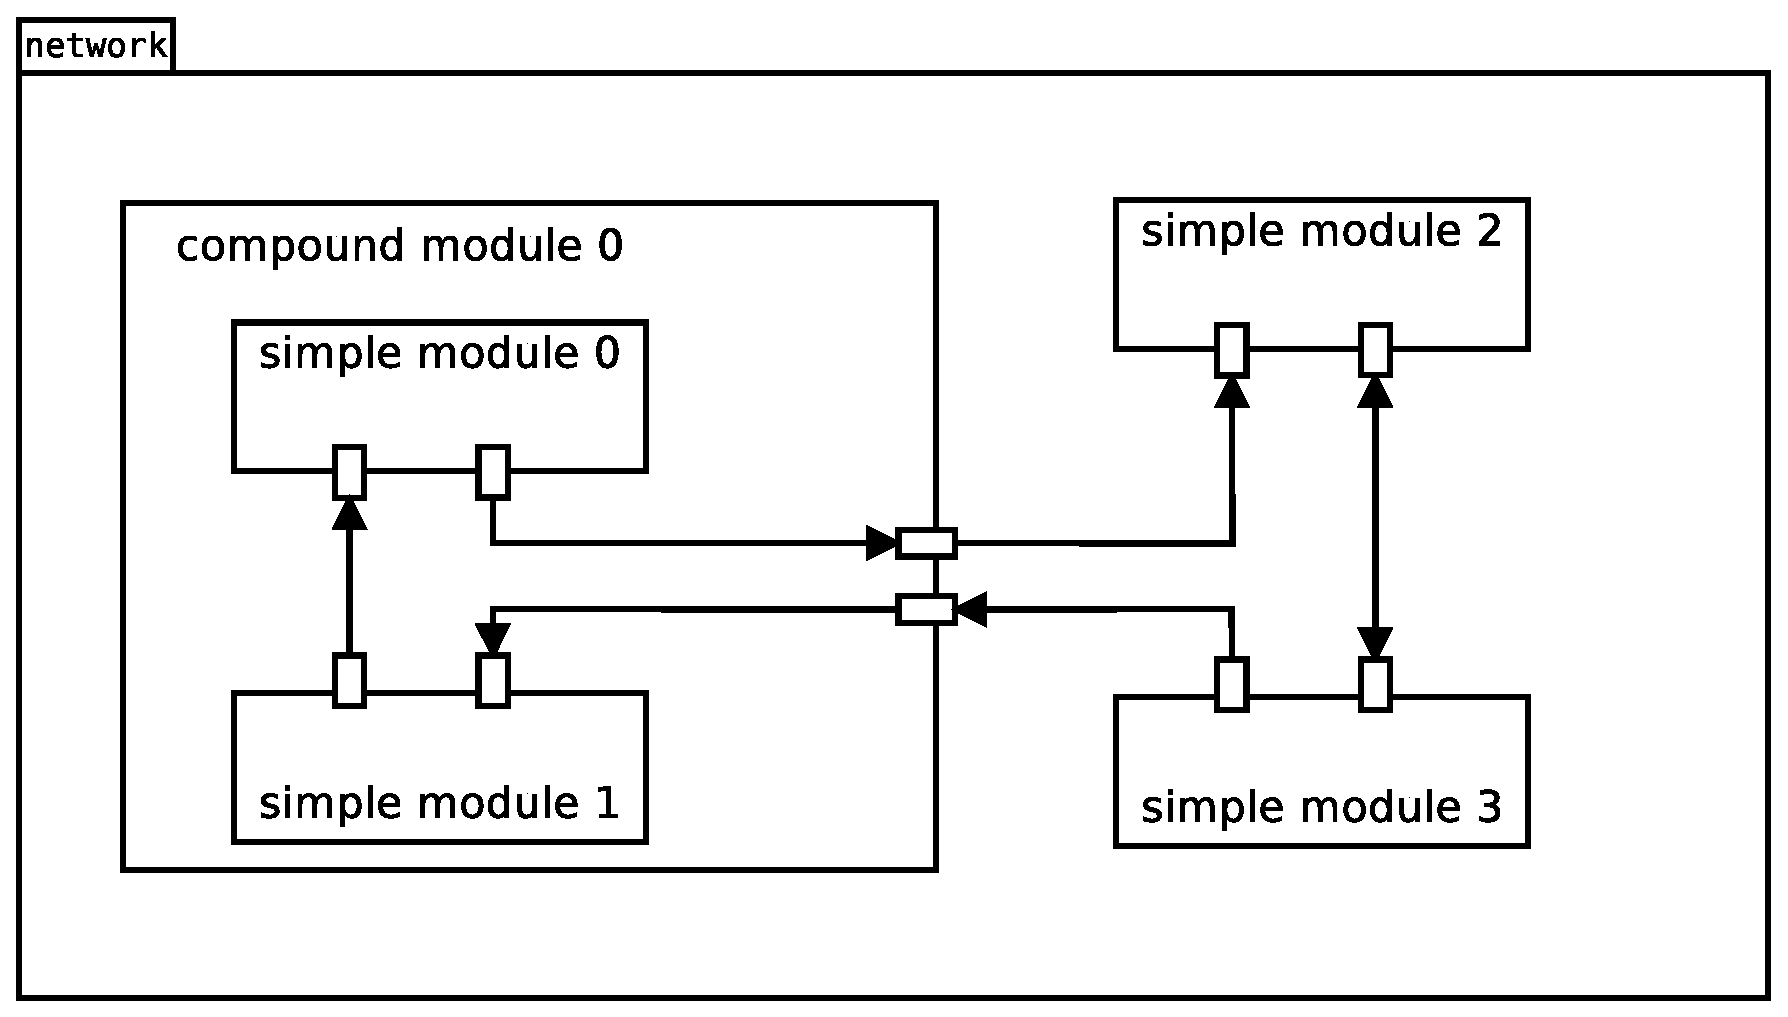
\includegraphics[width=0.9\columnwidth]{OMNeTComponents.eps}
    \caption{OMNeT++ components in an example network}
    \label{fig:OMNeTComponents}
\end{figure}

Each custom module and channel is defined in the \emph{NED} language.
Specific functionality for custom components is implemented in the according C++ code.
This assignment is usually done with identical names of the \emph{NED} file and the C++ code.
Examples and the combination of \emph{NED} files and C++ code is shown in \cite[chapter 3, chapter 4]{OMNETMANUAL}
The components can embed any functionality implemented in C/C++.
The usage of external libraries or language features is not limited, but must be used with care due to the effect on simulation performance.


\subsection{Messages}
Transmitted data are encapsulated in another component called messages.
Messages are a fundamental component of a OMNeT++ simulation as they does not only transport data they can also represent functional messages like jobs, events or tasks.
The meaning behind a message is depending on the written simulation and the simulated system.

These messages can also be customized for holding a specific set of data like a protocol header, checksum, etc. or other specific data.
The existing Message class \emph{cMessage} and its derived specialization \emph{cPacket} provide different Members and functions which can be used for simulations.
These include control information, type information, time stamp, etc. and are included for making developing a simulation easier.
Adding a few simple datafields to a Message can be ether done by subclassing \emph{cMessage} or \emph{cPacket} or using the \emph{NED} syntax.
By defining a custom Message using \emph{NED} a customized subclass will be generated by the simulation and can be normally used as Message.

Any module can send a message via a connected channel for this sent message a time is defined.
This time describes the moment when the message should be sent to the channel.
The mechanism of messages is also used for implementing timeouts, timers, etc. by sending a specific message to the current module, this is a so called \emph{self-message}.
These \emph{self-message} is handled by the same function as any other message coming from other modules.
For the identification of \emph{self-messages} there is a built in function available.
More information about messages and the possibilities of customized messages are given in \cite[chapter 5]{OMNETMANUAL}

Each message sent ether by another module or by the current module itself represents an event for the simulation with an according time, at which this event should happen, or the message should be delivered/received.
The execution and the handling of such created events is done by the simulation core and defines the execution order and the performance of the simulation.
Handling these events can be done in various ways and define the type of implemented simulation.
These simulations based on events are event based discrete simulations, the definitions of this type and the explanation of different simulation types are shown in the next section.

\section{Simulation}
\label{sec:Simulation}
Simulation can be done in different ways. The general categories are \emph{discrete} and \emph{continuous} simulations.
The difference is shown in the processing of the simulated systems and the handling of simulation time.

For continuous simulations the state of the simulated system can change at any time, therefore the complete simulated time range has to be executed.
This executions requires the definitions of a resolution and the calculation of each moment within the time range.

This requirement is not necessary for discrete simulations, because these simulations are event based.
For each event a time is specified at which the event has to be executed or handled.
For discrete simulations the system state is constant between two consecutive events and therefore this time can be skipped in simulation time.
The calculated moments within the simulation time are defined by the schedules events and their execution time.
%TODO: find reference for simulation type

Simulations written with OMNeT++ are by default discrete event based simulations.

\subsection{Event simulation}
\label{sec:EventSimulation}
Such simulations handle given events at the defined point in the simulation time.
The execution of the event takes no simulation time.
Each event processed in the simulation is handled at the exact simulation time which is defined individually.
This type of simulation enables simulating various events even within a very short simulated time range.

Within OMNeT++ this time is called \emph{arrival time}.
Each message contains the \emph{arrival time} and the \emph{sending time}, both are time points in the simulation time.
The \emph{sending time} is used for calculation of transmissions.
For the execution and handling of an event the \emph{arrival time} is more important.
Events are created by modules and then inserted in the so called future event structure (\emph{FES}).
The simulation core executes all events within the \emph{FES} at the according simulation time.

The main part of the simulation core of OMNeT++ which controls the event handling is the scheduler.
This scheduler accesses the \emph{FES} and chooses the next event to be handled by the simulation.
The class \emph{cScheduler} represents the interface which is required for a event scheduler usable in OMNeT++.
By default the derived class \emph{cSequentialScheduler} is used.
This scheduler implements the default discrete event based simulation and handles the events according to their execution time, scheduling priority and scheduled time.
The scheduling priority provides a mechanism for controlling the execution order of multiple events at the same time.
The functionality and the ordering of executed event by the \emph{cSequentialScheduler} are explained in \cite[section 4.1]{OMNETMANUAL}.

Approaching the field of emulation and \emph{HiL} the discrete event based simulation is unusable.
For such applications the type of real time simulation is required.

\subsection{Real time simulation}
\label{sec:RealTimeSimulation}
Real time simulations change the meaning of simulation time.
The simulated events should be executed at the correct time to match the real time.
In this context \emph{the real time} means the real world time, cpu time, or wall time, i.e. the time which passes for the real world during the execution of the simulation.
This type of simulation is not possible for every simulated systems as the limits are defined by the execution speed of the host system.
Achieving this match of simulation time and real time is strongly depending on the targeted time resolutions and time spans between events.
The needed time for calculating new events and reacting to incoming events is defined by the executed functions and is therefore defined by the simulated system.
Lightweight simple modules with plain functions can be simulated with faster event frequencies than compound modules consisting of multiple modules with complex behavior.

Approaches for achieving this type of simulations are implemented in the \emph{cRealTimeScheduler} within OMNeT++.
This Scheduler executes the events according to their planned arrival time.
The arrival time of the next event is compared with the current real time.
When the simulation is ahead of the real time, the simulation is paused for the remaining time.
The \emph{cRealTimeScheduler} waits in hard-coded 100 ms chunks for achieving a responsive simulation.
For emulations and \emph{HiL} this concept is not applicable, because the communication with real components does not allow a sleep time.
The OMNeT++ sample \emph{sockets} demonstrate this problem and a possible solution with a custom scheduler implementing the \emph{cScheduler} class.
This custom scheduler named \emph{SocketRTScheduler} listens to the interface during the times when the simulation has to wait until the next event should be executed.
This allows the receiving of packets from real clients and the connection of the simulated components with real ones.
The implementation of \emph{SocketRTScheduler} is not fully optimized and is intended to show the possibility of emulation and \emph{HiL} using OMNeT++.

Handling the difference for a simulation which is faster than the real world system can be done in various ways as demonstrated by \emph{cRealTimeScheduler} and \emph{SocketRTScheduler}.
The implementation of the scheduler and a description of their functionality can be found in the OMNeT++ sources and samples or in the API reference \cite[]{OMNETAPIREF}.

Is the simulation lagging behind the real time, the scheduler must try to speed up the simulation and catch up to the real time.
The \emph{cRealTimeScheduler} executes the next events immediately and therefore skipping sleep times.
With this behavior the task of catching up to the real time becomes very difficult for complex simulations with tight timings.
Lags the simulation constantly behind the real world using the \emph{cRealTimeScheduler} it becomes discrete event based.

The achieved simulation time can be defined by the performance ratio which can be shown during simulation.
This ration represents the simulated seconds per real time seconds.
A lagging simulation is defined by a performance ration of less than 1 and simulation which simulates faster as the real time shows a ratio of greater than one.
The goal of a real time simulation is a constant ratio of 1.
The process of catching up by a lagging simulation and achieving a performance ratio of 1 can also influence other timings.
Therefore the variation of delays (jitter) increases when the simulation lags temporarily.
For emulations and the field of \emph{HiL} a increased jitter for a signal can be very critical and must be analyzed carefully.

The host machine for the simulation and its components affect the achieved simulation times.
The dependencies of the host system and the result of existing researches is shown in section \ref{sec:SystemDependencies}.

Developing the simulation of a given system results in the situation of many provided code which should be executed depending on incoming messages and therefore creating new message for sending.
Given systems can be designed in various hierarchies in sight of number of modules and complexity of simple modules.
The different designs and their effect on real time simulation is shown in the next section.

\section{Module design}
\label{sec:ModuleDesign}
Implementing a simulation of a given system brings up different design questions regarding complexity of modules and the designed hierarchy.

\subsection{Modular design}
Designing a granular system in OMNeT++ with a bigger number of modules connected with channels and grouped in compound modules allows a more dynamic simulation and can increase the reuse-ability of modules.
This approach is convenient for simulating deep features and procedures within systems.
When a simulated system or network consists of multiple systems such a design can be problematic in sight of communication and simulation overhead.
Approaching emulation and the field of \emph{HiL} using the real time simulation these design decisions are important for the achieved timings.

A example of a modular design is shown in figure \ref{fig:OMNeTModularDesign}.

\begin{figure}
    \centering
    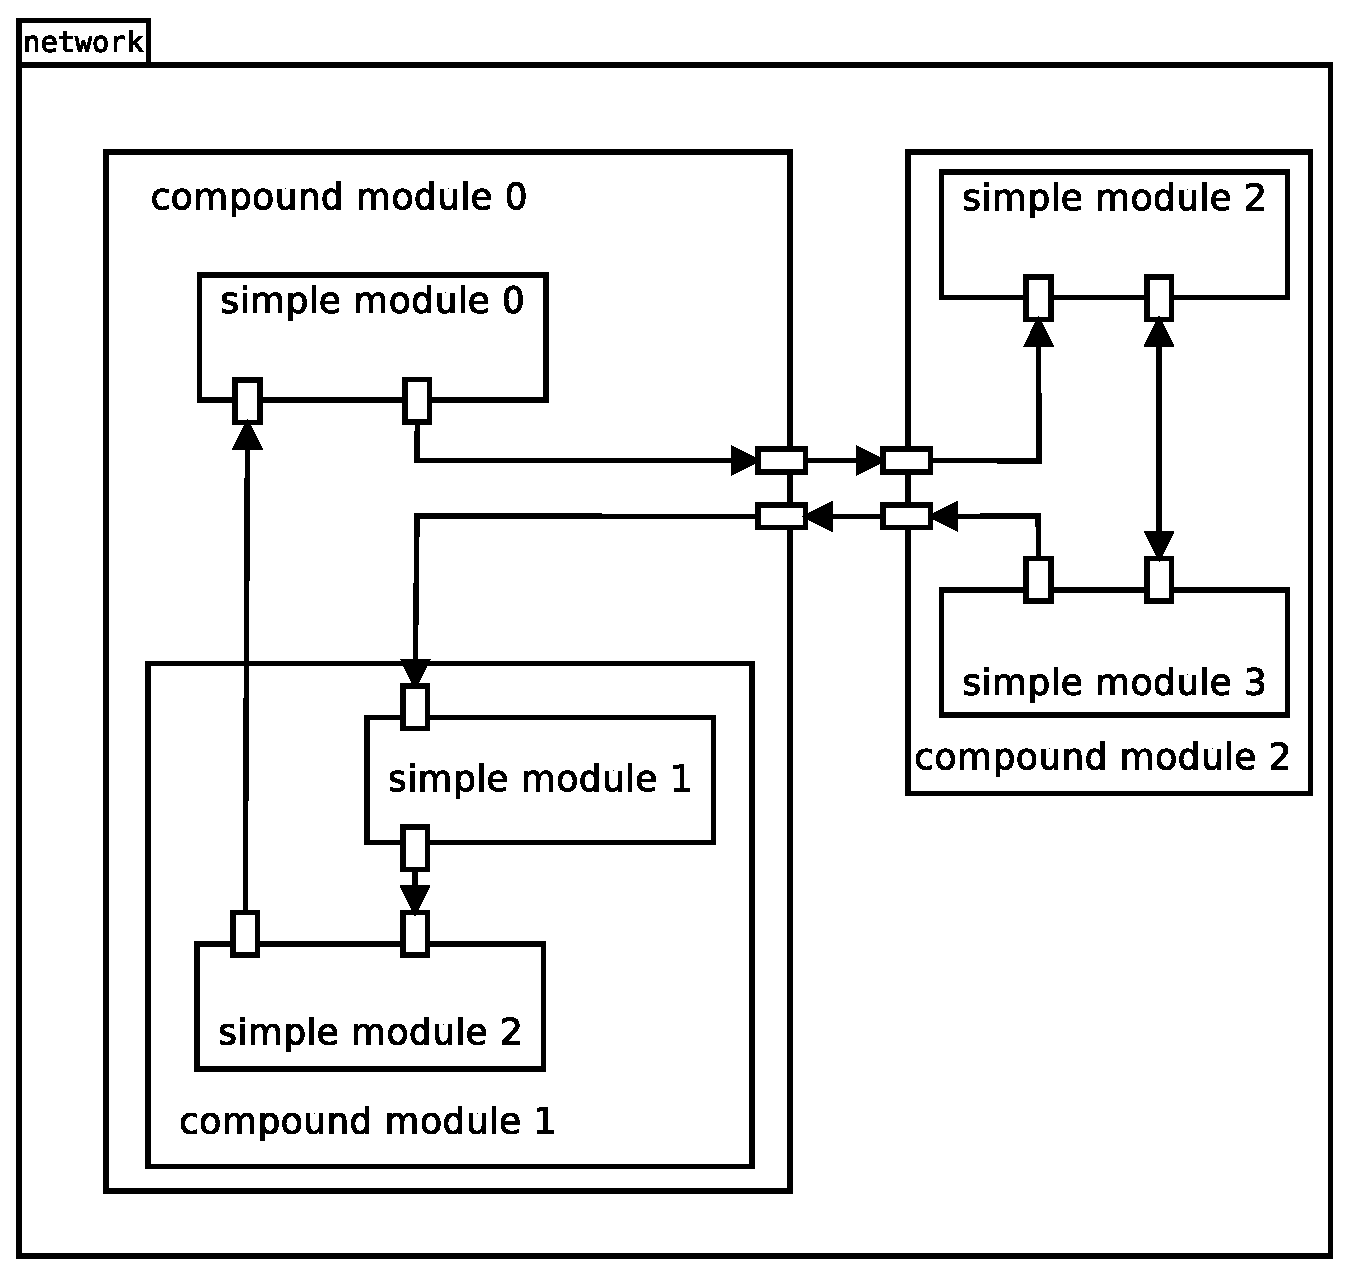
\includegraphics[width=0.9\columnwidth]{OMNeTModularDesign.eps}
    \caption{Modular design with OMNeT++}
    \label{fig:OMNeTModularDesign}
\end{figure}

\subsection{Monolithic design}
Decreasing the overhead of communication and simulation can be achieved for example by condensing a compound module to a simple module with more complex functions to execute.
This leads to a monolithic design containing less modules with more complex functions.
The execution of the single modules include more normal C++ code using simple method calls and operations.

The previous example network showing a modular design in figure \ref{fig:OMNeTModularDesign} can be condensed to a more monolithic design.
In the example, shown in figure \ref{fig:OMNeTMonolithicDesign}, the compound modules 0 and 2 with all their submodules were replaced by two simple modules.
The channels and the sent messages between the modules stay the same, but the calculation within the modules include the complete behavior of the previously included components.

\begin{figure}
    \centering
    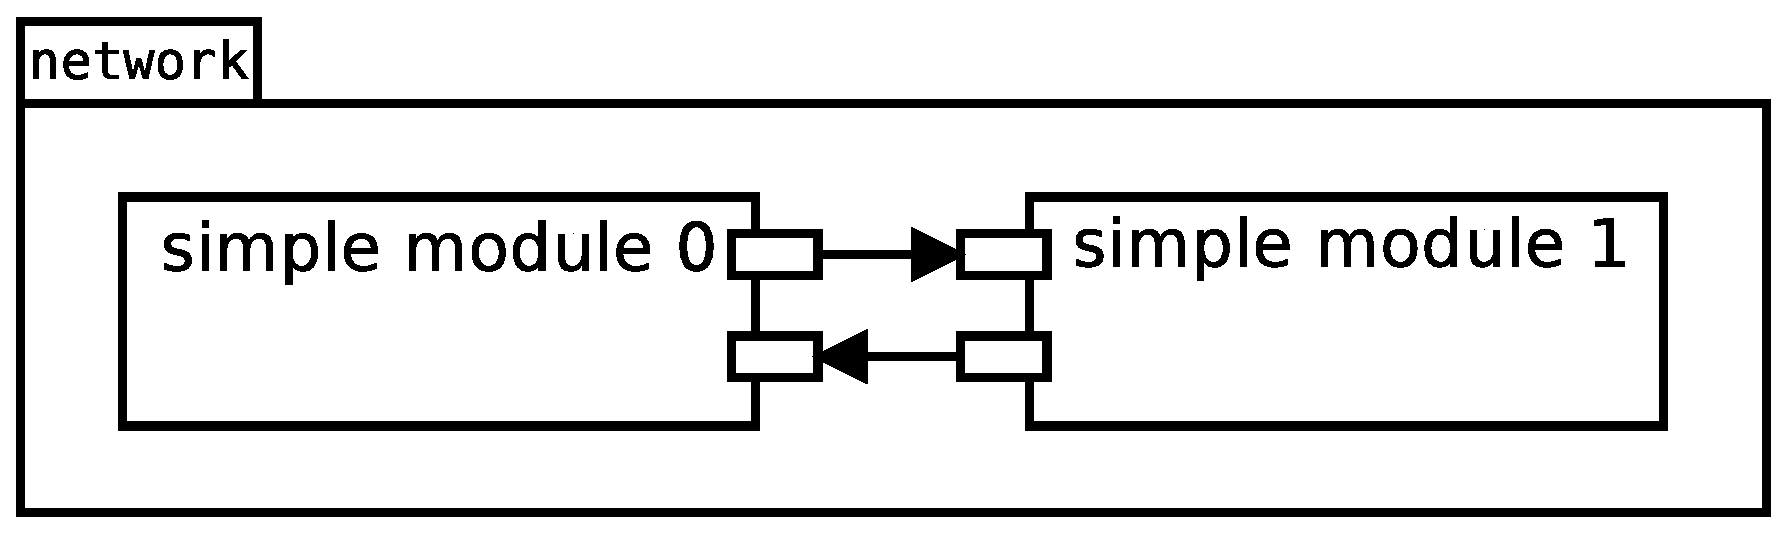
\includegraphics[width=0.9\columnwidth]{OMNeTMonolithicDesign.eps}
    \caption{Monolithic design with OMNeT++}
    \label{fig:OMNeTMonolithicDesign}
\end{figure}

\section{System dependencies}
\label{sec:SystemDependencies}
The host system for the simulation is very important regarding simulation speed and achievable timings of a real time simulation.
As described in \cite{Sekercioglu2003} OMNeT++ is capable of running a parallel simulation when specific requirements are met.
Running the simulation parallelized can achieve better timings and increase the possibilities of real time simulations.

% needed in second column of first page if using \IEEEpubid
%\IEEEpubidadjcol


% An example of a floating figure using the graphicx package.
% Note that \label must occur AFTER (or within) \caption.
% For figures, \caption should occur after the \includegraphics.
% Note that IEEEtran v1.7 and later has special internal code that
% is designed to preserve the operation of \label within \caption
% even when the captionsoff option is in effect. However, because
% of issues like this, it may be the safest practice to put all your
% \label just after \caption rather than within \caption{}.
%
% Reminder: the "draftcls" or "draftclsnofoot", not "draft", class
% option should be used if it is desired that the figures are to be
% displayed while in draft mode.
%
%\begin{figure}[!t]
%\centering
%\includegraphics[width=2.5in]{myfigure}
% where an .eps filename suffix will be assumed under latex, 
% and a .pdf suffix will be assumed for pdflatex; or what has been declared
% via \DeclareGraphicsExtensions.
%\caption{Simulation Results}
%\label{fig_sim}
%\end{figure}

% Note that IEEE typically puts floats only at the top, even when this
% results in a large percentage of a column being occupied by floats.


% An example of a double column floating figure using two subfigures.
% (The subfig.sty package must be loaded for this to work.)
% The subfigure \label commands are set within each subfloat command, the
% \label for the overall figure must come after \caption.
% \hfil must be used as a separator to get equal spacing.
% The subfigure.sty package works much the same way, except \subfigure is
% used instead of \subfloat.
%
%\begin{figure*}[!t]
%\centerline{\subfloat[Case I]\includegraphics[width=2.5in]{subfigcase1}%
%\label{fig_first_case}}
%\hfil
%\subfloat[Case II]{\includegraphics[width=2.5in]{subfigcase2}%
%\label{fig_second_case}}}
%\caption{Simulation results}
%\label{fig_sim}
%\end{figure*}
%
% Note that often IEEE papers with subfigures do not employ subfigure
% captions (using the optional argument to \subfloat), but instead will
% reference/describe all of them (a), (b), etc., within the main caption.


% An example of a floating table. Note that, for IEEE style tables, the 
% \caption command should come BEFORE the table. Table text will default to
% \footnotesize as IEEE normally uses this smaller font for tables.
% The \label must come after \caption as always.
%
%\begin{table}[!t]
%% increase table row spacing, adjust to taste
%\renewcommand{\arraystretch}{1.3}
% if using array.sty, it might be a good idea to tweak the value of
% \extrarowheight as needed to properly center the text within the cells
%\caption{An Example of a Table}
%\label{table_example}
%\centering
%% Some packages, such as MDW tools, offer better commands for making tables
%% than the plain LaTeX2e tabular which is used here.
%\begin{tabular}{|c||c|}
%\hline
%One & Two\\
%\hline
%Three & Four\\
%\hline
%\end{tabular}
%\end{table}


% Note that IEEE does not put floats in the very first column - or typically
% anywhere on the first page for that matter. Also, in-text middle ("here")
% positioning is not used. Most IEEE journals use top floats exclusively.
% Note that, LaTeX2e, unlike IEEE journals, places footnotes above bottom
% floats. This can be corrected via the \fnbelowfloat command of the
% stfloats package.



\section{Conclusion}
The conclusion goes here.





% if have a single appendix:
%\appendix[Proof of the Zonklar Equations]
% or
%\appendix  % for no appendix heading
% do not use \section anymore after \appendix, only \section*
% is possibly needed

% use appendices with more than one appendix
% then use \section to start each appendix
% you must declare a \section before using any
% \subsection or using \label (\appendices by itself
% starts a section numbered zero.)


% Can use something like this to put references on a page
% by themselves when using endfloat and the captionsoff option.
\ifCLASSOPTIONcaptionsoff
  \newpage
\fi

% trigger a \newpage just before the given reference
% number - used to balance the columns on the last page
% adjust value as needed - may need to be readjusted if
% the document is modified later
%\IEEEtriggeratref{8}
% The "triggered" command can be changed if desired:
%\IEEEtriggercmd{\enlargethispage{-5in}}

% references section
\printbibliography

\end{document}


